\section{System design}
% Hvilke problemer er der ved systemet?
%Systemet skal kunne lagre og indlæse beskeder til og fra et eksternt socialt medie, hvilket vil spille den stor rolle i 
% Beslutninger
% Fokus på kravene, nævn dem med nummerering
% Måske som separat latex section
% let oprids af de etiske dilemmaer i projektet
% teknologierne
% det sociale medie som et mellemled, for at steganografere beskederne i mængden af meget andet indhold
Ud fra kravspecifikationen bliver systemet pålagt at være sikkert, men samtidig også at køre med en fornuftig indlæsnings tid. Disse krav kan  modarbejde hinanden på flere forskellige måder, blandt andet i spørgsmålet om systemet skal køre centralt eller decentralt.

\subsection{Central eller decentral løsning}
Hvis man har spørgsmålet med optimal indlæsnings tid i mente, så vil en central løsning med en server der lagrer stien til alle beskeder i systemet. Dette gør enheder der tilgår den centrale database i stand til at forespørge og finde opslag meget hurtigt, da den har kortlagt alle relevante opslag. Dette står i modsætning til en decentral løsning, hvor brugernes enhed fungerer som mikro servere der selv skal søge efter de relevante opslag. Den søgning kræver langt flere server anmodninger decentralt, da den centrale kortlægning ikke er tilgængelig. De mange anmodninger vil resultere i længere indlæsnings tid.

\begin{figure}[H]
    \begin{subfigure}{0.5\textwidth}
        \centering
        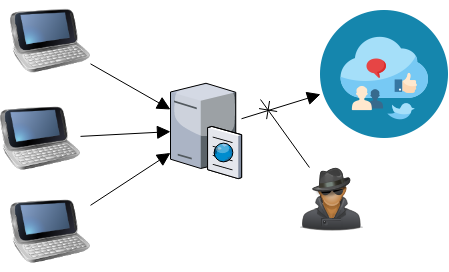
\includegraphics[width=1\linewidth, height=4cm]{Projectdoc/Assets/Illustrationer/Security_diagram_1.png} 
        \caption{Central server}
        \label{fig:central_server}
    \end{subfigure}
    \begin{subfigure}{0.5\textwidth}
        \centering
        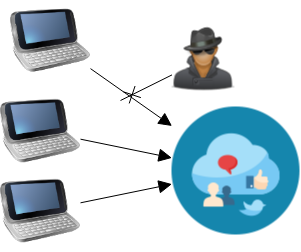
\includegraphics[width=0.7\linewidth, height=4cm]{Projectdoc/Assets/Illustrationer/Security_diagram_2.png}
        \caption{Klient-baseret system (decentral)}
        \label{fig:decentral_server}
    \end{subfigure}
    \caption{Forskellen på central og decentral server struktur}
    \label{fig:serverstruktur}
\end{figure}

En central server trods dens eventuelle positive egenskaber, udgøre dog også et potentielt sikkerhedshul, hvis denne server ikke er sikret tilstrækkeligt. Med andre ord lægger dette en systemvedligeholdelse byrde på dem der administrerer systemet. F.eks. kunne en sådan server, (Illustreret ved [Figur \ref{fig:central_server}]), lække generelle lagerede informationer, eller ligefrem blive overvåget for kommunikation, samt blive spærret som en helhed. Dette vil selvfølgelig også kunne ske for den enkelte bruger [Figur \ref{fig:decentral_server}], men disse ville i sådanne tilfælde også kun påvirke den enkelte, og ikke systemet som en helhed.
\\\\
%\textbf{Argumenterne for en delvis decentral løsning}\\
Jo mere et givet system afhænger af bestemte nodes, jo vigtigere er det at sikre disse nodes, både i forhold til DoS angreb, men også i forhold til kompromittering af bruger data. På den anden side, vil anvendelsen af servere i et centralt systemet også tillade en langt højere effektivitet. Derfor vil forskellige aspekter af kommunikationsplatformen blive videre diskuteret for at kunne finde et kompromis mellem helt centraliseret og helt decentraliseret.\\

\begin{figure}[H]
    \begin{subfigure}{0.33\textwidth}
        \centering
        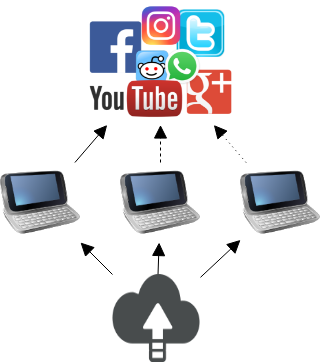
\includegraphics[width=0.7\linewidth, height=4cm]{Projectdoc/Assets/Illustrationer/Device_Opdate.png} 
        \caption{Lokale device kendte lister, opdateret med software opdateringer}
        \label{fig:DeviceOpdate}
    \end{subfigure}
    \begin{subfigure}{0.33\textwidth}
        \centering
        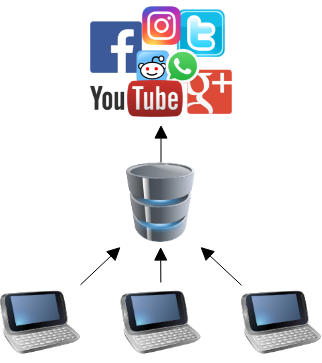
\includegraphics[width=0.7\linewidth, height=4cm]{Projectdoc/Assets/Illustrationer/CentralDatabase.png}
        \caption{Central Database}
        \label{fig:CentralDatabaseList}
    \end{subfigure}
    \begin{subfigure}{0.33\textwidth}
        \centering
        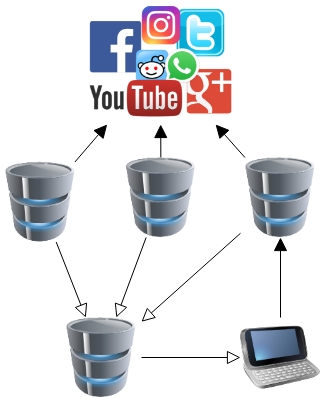
\includegraphics[width=0.7\linewidth, height=4cm]{Projectdoc/Assets/Illustrationer/MainDomainServer.png}
        \caption{Flere Databaser, kendt af devices, og opdateret fra en hoved database}
        \label{fig:MainDomain}
    \end{subfigure}
    \caption{Forskellige medie kontakt former.}
    \label{fig:MedieContact}
\end{figure}

For at kunne opretholde en mængde af bots, her forstået som anonyme brugere på sociale medier genereret af systemet, der har til opgave at sikrer anonymitet for brugeren på kommunikationsplatformen, associeret med en potentielt mistænkelig opførelse, vil det være nødvendigt at kunne tilføje nye bots til netværket løbende, samt opdatere status af nuværende bots, da det kunne formodes at ejerne af det relevante sociale medie ikke ønsker systematisk genereret anonyme brugere. Én mulig måde at holde styr på disse informationer kunne være, som illustreret ved [Figur \ref{fig:CentralDatabaseList}]. En database opdateret med information om de enkelte bots på de sociale medier, omhandlende om de stadigvæk er aktive, eller om de er blevet banlyst af det sociale medie, f.eks. for ikke at være en "normal" bruger. Hvis en given bot så blev lukket ned, ville den opdaterede database, gøre enhver bruger i stand til blot at vælge en anden bot. Denne løsning tilfører dog et element, en database, som vil være et kritisk led i, at tilbyde yderligere anonymitet til brugeren. Hvis denne database så ikke er tilgængelig, ville denne funktionalitet være hindret, i det at bots vil kunne blive taget ned i mellemtiden, uden at brugeren vil vide det, før brugeren får en fejlmeddelelse. Endnu værre kunne kompromitteringen af denne database gøre det muligt for uvedkommende at læse beskederne sent igennem systemet. Dette vil især være væsentligt hvis der er anvendt kryptering som ekstra sikkerhed på beskederne. Disse krypteringsnøgler vil så skulle gemmes et sted hvor alle de egentlige bruger kan få fat i dem. Derfor vil sikringen af sådan en database være vigtig. Såfremt denne database kun kontaktes for at få listen opdateret, vil trafikken imellem den og klienterne dog være begrænset. Man kunne også forestille sig en ekstra database, som illustreret ved [Figur \ref{fig:MainDomain}], der kun vil blive kontaktet hvis den primære er inaktiv, og at denne database kender til andre databaser, der opererer som backups af den primære. Denne opbygning vil gøre det meget svært at lukke systemet i længere tid. På den anden side vil dette opsætning også kræve mere hardware og mere vedligehold i form af synkronisering, opdatering osv. Dermed vil en opsætning af en sådan backup koste systemadministratoren mere arbejdstid, og vil derfor kræve en vurdering af, om opsætningen er investeringen værd.\\
En måde at undgå dette databaseproblem, er at lade hver klient have en lokal liste over aktive bots, som illustreret ved [Figur \ref{fig:DeviceOpdate}]. Denne liste vil så med jævne intervaller blive opdateret igennem klient opdateringer. Med denne fremgang er det tænkeligt, at systemet vil kræve mange opdateringer, eller at der ofte vil være et antal utilgængelige bots på listen, i denne illustration vist ved de mere ødelagte forbindelser.
\\\\
%\textbf{Argumenterne for en central løsning}\\
Som førnævnt vil et centraliseret system betyde at hele systemet vil hvile på en node, hvilket vil betyde at en angriber blot skal tage et led ud for at kollapse hele systemet. En måde hvorpå man kunne sikre systemet under en central server, er ved at lagre krypteringsnøgler på serveren, der skal hentes for at kunne læse en besked. Denne centrale server bliver det eneste led som en ondsindet angriber skal lægge ned, for at gøre hele platformen ubrugelig. Dette vil faktisk sikre brugerne, såfremt angriberen ikke kompromitterer krypteringsnøglerne. Brugernes beskeder vil være ulæselig for en angriber uden de krypteringsnøgler. Dette kan sammenlignes med en indbygget selvdestruktion af systemet.\\
Et centraliseret system vil altid kunne opdateres løbene, i modsætning til den decentraliseret løsning hvor brugerne enten er fastlåst med software der potentielt er defekt eller skal hentes på ny. Løbene opdateringer til systemet er essentielt når det sociale netværks bot konti der benyttes, ikke fungerer som tiltænkt. Dette kan ske på mange forskellige måder: Blandt andet kan de enkelte bots blive taget ned for mistanke for falsk bruger, eller netværket kunne ændre sin struktur fra en ene dag til den anden. Muligheden for løbene opdatering er også essentiel ved en mulig skalering af systemet, blandt andet når systemets netværk af bots ikke kan betjene en voksene brugerbase, eller når denne brugerbase ændret behov der kræver at det fundamentale system gennemgår strukturel redesign.
\\\\
\textbf{Samlet konklusion}\\
Selvom en komplet decentraliseret løsning lyder godt på papiret, så vil det udløse så mange fundamentale problemer at systemet vil være bøvlet og potentielt ubrugeligt. Da systemet afhænger så kraftigt på en trejdeparts service, så vil små ændringer så som:
\begin{itemize}
    \item[-] Systemets bot netværk kan blive delvist eller helt lukket ned. Dette kan ske af mange forskellige grunde blandt andet ved brud på det sociale medies ToS (Terms of Service) eller ved en eventuel afsløring af hele systemet / projektet. 
    \item[-] Tredjeparten kan ændre deres API struktur på sådan vis at det fundamentale system ikke længere fungerer som tiltænkt.
    \item[-] Ved en decentral løsning vil det ikke være muligt at lukke alle brugernes tilgang på samme tid, da der ikke er nogen central database som knudepunkt.
    \item[-] Det vil kræve løbende opdatering af klienterne, at holde listen af aktive bots fuldt funktionel.
    \item[-] I en løsning med en central server, vil det være muligt at løbende holde styr på nye tråde og tilføjelser til eksisterende tråde. Dette ville skåne brugeren for en stor del ventetid.  
\end{itemize}

% teknisk svær opgave

\subsection{Sammenkædning af beskederne}
På projektets sikrede kommunikationsplatform vil det være nødvendigt at kunne finde sammenhængende beskeder og denne sammenkædning vil ikke kunne foregå på åbenlys vis på et socialt medie. I stedet kunne én mulighed være, at gemme sammenhængen i noget tilsyneladende uskyldig metadata, men som er genereret ud fra en prædefineret algoritme. Dette vil give den sikrede kommunikationsplatform noget specifikt at søge efter, uden at det vil være et let læseligt flag. Men hvad er metadata?\\\\
Metadata kan grundlæggende defineres som data om data. Dermed kan det anvendes i mange sammenhænge. Et eksempel kunne være et billede. Dataen i et billede er i simpleste forstand lysintensiteter, i sort/hvid billeder, eller farver. Men udover denne data kunne man også gemme ting som dato, klokkeslet, GPS koordinater, navnet på ophavsmanden osv. Alt dette er eksempler på metadata som ikke påvirker indholdet, men som gør indholdet mere brugbart i mange forskellige sammenhænge. For eksempel vil vedhæftede søgeord gøre et billede galleri meget mere effektivt i at præsentere det ønskede materiale. Metadata kan både genereres automatisk af hardware/software systemer, men en bruger kunne også tilføre metadata manuelt.\\ Dette er især sandt på sociale medier hvor der kan findes en stor mængde af generelle søgeord. Netop det faktum at sociale medier tillader de enkelte brugere at skabe en varierende mængde af metadata for et hvert billede, sandsynliggør at systemet vil være i stand til at generere disse søgeord med en prædefineret algoritme for hver tråd på forummet. Dette vil så gøre det muligt at søge efter nye opslag på enhver forumstråd.
\\\\
\textbf{Forum struktur}\\
Da et forum kan designes på flere måder vil det her blive diskuteret hvordan det bedst vil passe til produktets tænkte anvendelse.

\begin{figure}[H]
    \begin{subfigure}{0.5\textwidth}
        \centering
        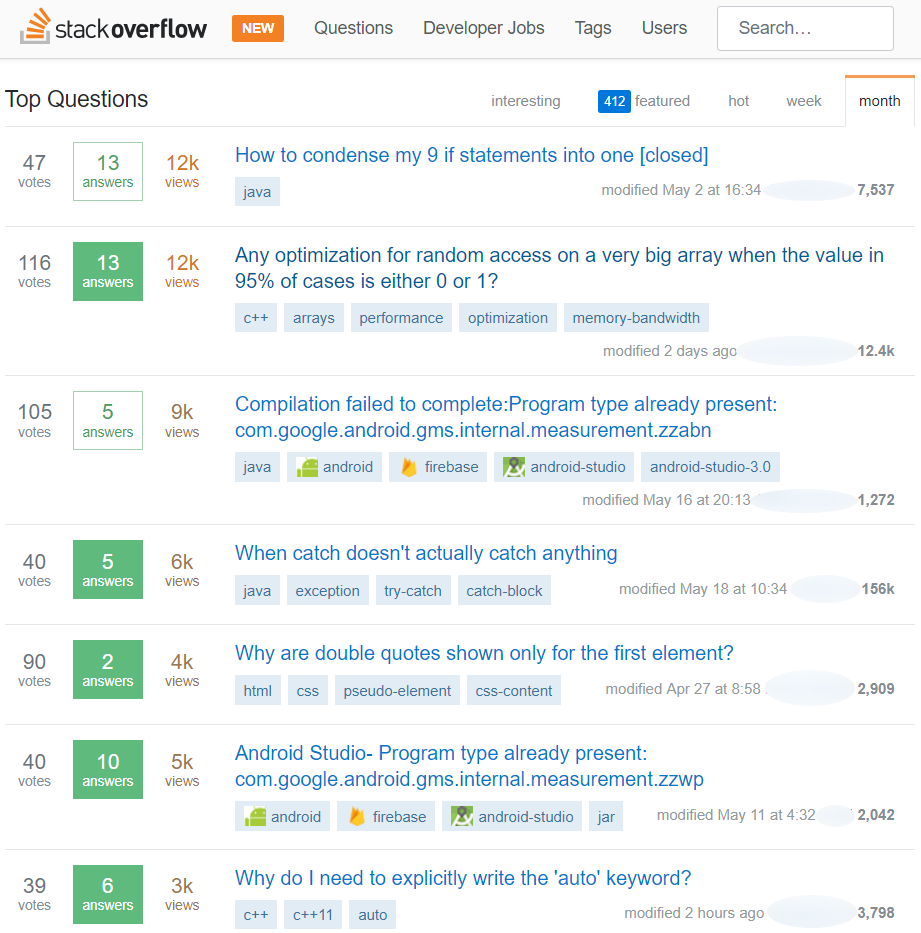
\includegraphics[width=1.0\linewidth ]{Projectdoc/Assets/Illustrationer/stackoverflow_forum_eksempel.png} 
        \caption{Stackoverflow forum struktur}
        \label{fig:stackoverflow_forum}
    \end{subfigure}
    \begin{subfigure}{0.5\textwidth}
        \centering
        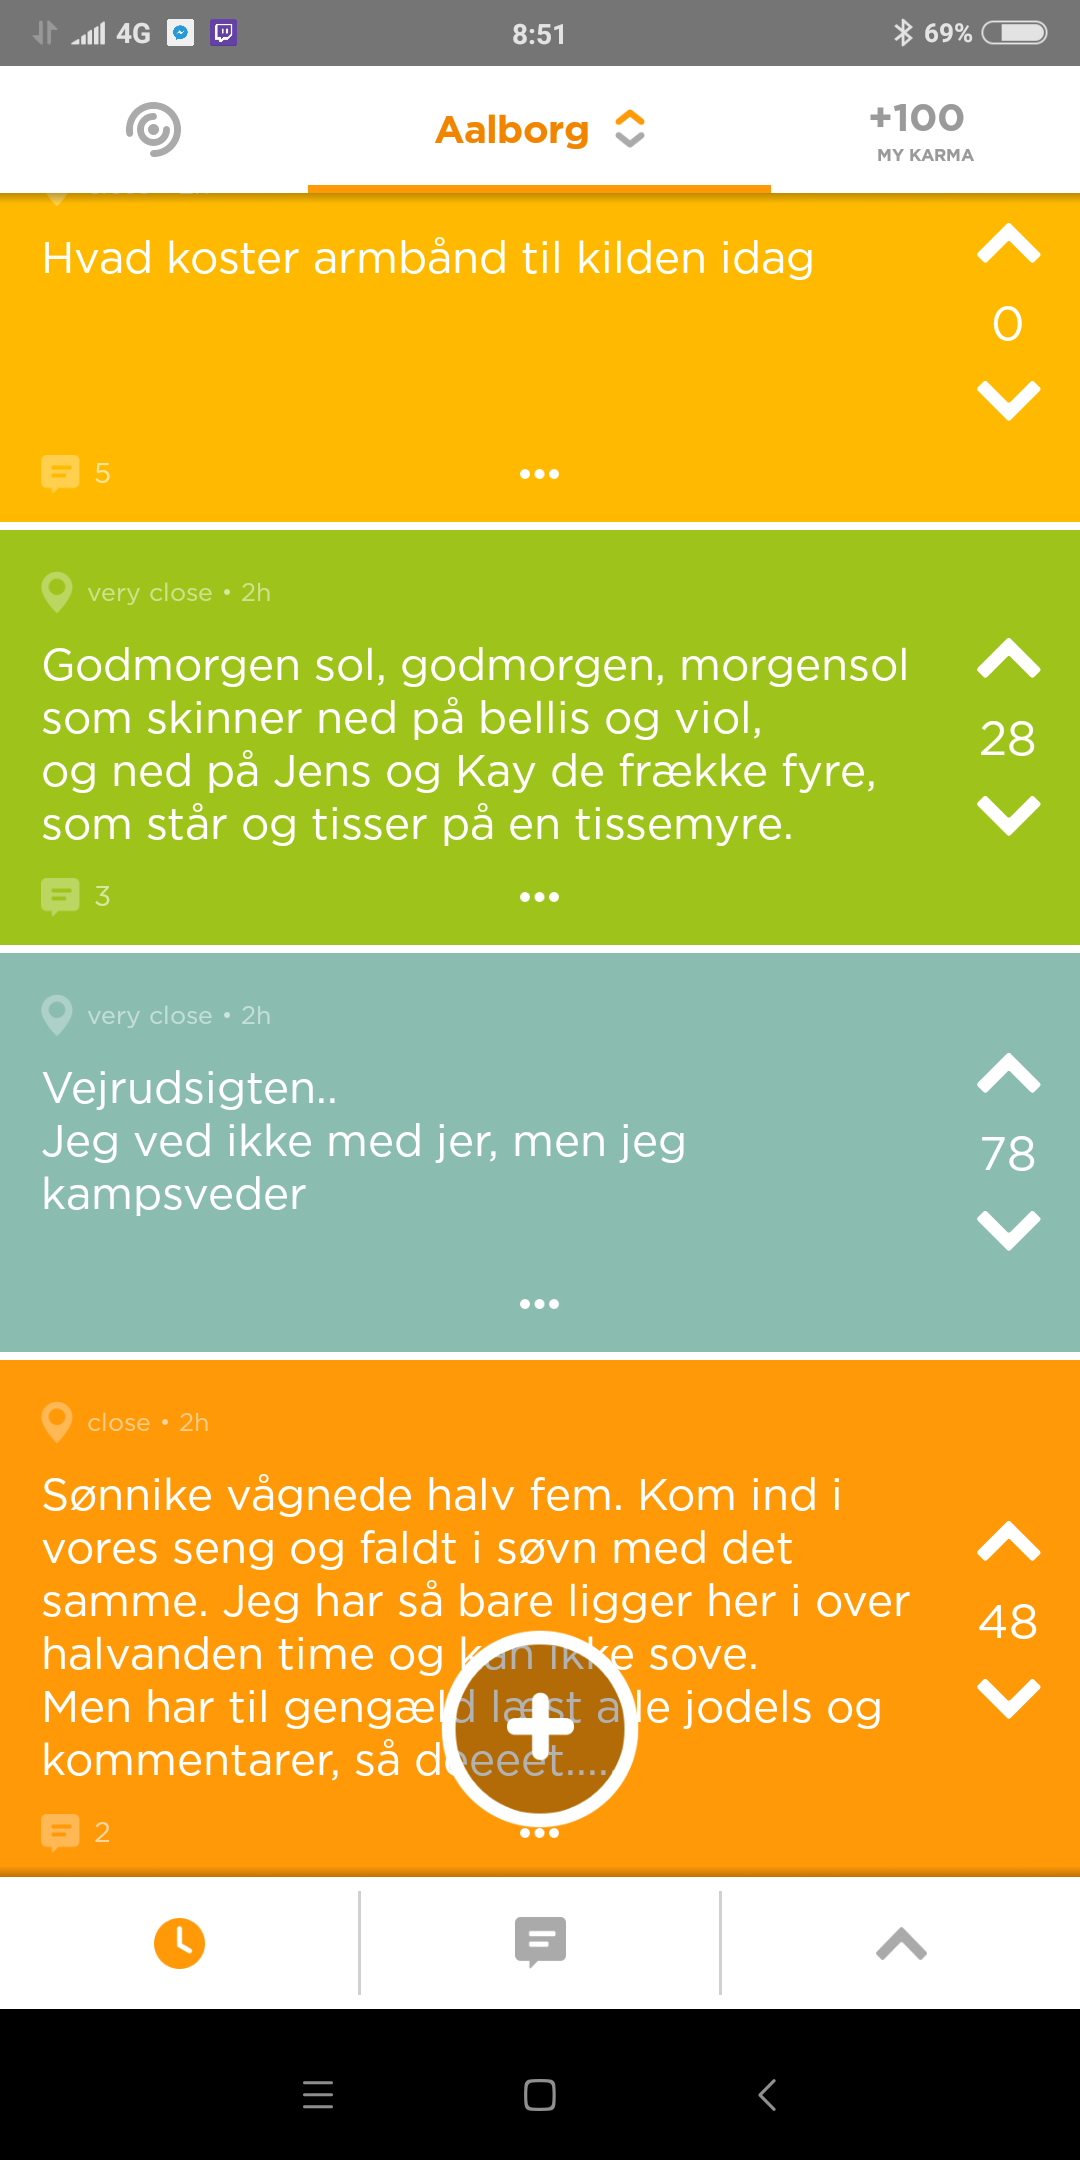
\includegraphics[width=0.8\linewidth]{Projectdoc/Assets/Illustrationer/jodel_forum_eksempel.png}
        \caption{Jodel forum struktur}
        \label{fig:jodel_forum}
    \end{subfigure}
    \caption{Forskellige fora}
    \label{fig:forskellige_fora}
\end{figure}

% Giv eksempler på meta på sociale medier --- 


% Hvordan skal forum strukturen være?
% - Jodel agtigtigt. Alle tråde på en lang række.
% - Forum med definerede kategorier med tråde.

% Foruden selve strukturen: Er der også problemer med fetching af sammenhæng? - Kædning til næste afsnit
\\
\textbf{Køretid}\\
% - Hvordan kan man sikre en fornuftig køre tid? (Undg̊a 10000 undersøgelser for at finde  ́en kommentar)
% - Formindsk chancen for mistænkelig data trafik. B̊ade i server requests og det visuelt uploaded
% — Load tid

\\
\textbf{Private beskeder}\\
En feature der vil kunne sikre yderligere sikker for bestemte type bruger og brugsmål er muligheden for at sende private beskeder. 




% - Med kun bots
% -- Request mængde
% -- API afhængighed

% - Bruger login
% -- Bruger sikkerhed

% - Samlet løsning med måde bot og bruger



% Må man dele en social medie konto med flere mennesker?? ToS overvejelse

% Kan der være et kulturelt problem i steganografi på et socialt medie?

\subsection{Opsummering af alle overvejelserne}
Ud fra overstående overvejelser og metoder, kan et endeligt system dannes som følgende struktur.

\begin{figure}[H]
    \centering
    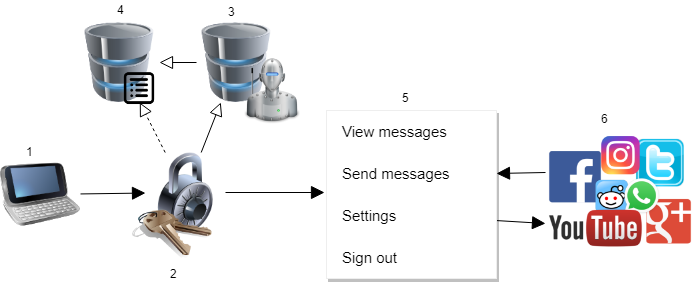
\includegraphics[width=0.70\linewidth]{Projectdoc/Assets/Illustrationer/System_struckure.png}
    \caption{System}
    \label{fig:sysdiagram}
\end{figure}

Systemets struktur beskriver, en central database [Figur \ref{fig:sysdiagram} . punkt 4] indeholdende information om alle systemet mindre database [Figur \ref{fig:sysdiagram} . punkt 3], der kan eksistere i uvist eller dynamisk antal, og videre indeholder informationer til anonyme bruger, om de aktive bots, der er dynamisk genereret til de enkelte sociale medier.
Denne centrale database er herved kun tilgået fra enddevices, når de ikke længere kan tilgå enkelte mindre databaser, symboliseret i [Figur \ref{fig:sysdiagram}] men stiplet linje, og har derfor ingen direkte forbindelse til omverdenen, ud over de enkelte enddevices. \\
Den centrale database kræver videre kun vedligeholdelse i dennes indhold, men til gengel kræver de mindre databaser opsætning for hver gang disse opdateres, efter eventuelle lukninger fra sociale medier, ligesom botsene dem selv også kræver det samme.
Devicene [Figur \ref{fig:sysdiagram} . punkt 1] kan herefter selv hente information, fra disse mindre databaser, nødvendig til at danne beskederne, og til sidst også selv poste eller helte beskeder, samt besked tråde, til/fra de sociale medier.

%Systemet beskrevet ved [Figur \ref{fig:sysdiagram}] er baseret på en brugers aktive handlinger, og %kan derved styres fra et centralt sted. Her tales om enten brugerens egen enhed, eller en central %server, der ikke fortager andre handlinger end at responderer klart på en brugers kommandoer.

%I systemets handlings diagram ovenfor [Figur \ref{fig:sysdiagram}] ses produktets overordnede handlingsflow. Diagrammet er ikke en endelig eller færdig udarbejdelse, men skabt til at give et letforståeligt overblik over systemets indhold, nødvendige resurse behov, samt mulige anvendte teknologier. Ud fra diagrammets flow, med start fra den sorte cirkel i toppen, kan der som et eksempel ses, at systemet anses for at skulle have tilgang til en Database, indeholdende mulige Bot associeringer til en brugeres login, eller en tilgang til det anvendte sociale medies API for samme.\\
%I dette eksempel er f.eks. ikke videre beskrevet hvordan, eller om systemet overhovedet skal, håndtere denne databases placering eller tilgang, efter en eventuel spærring fra tredjeparter, der f.eks. kunne anse systemet for at understøtte maliciøse aktiviteter.\\
%Efter denne login aktivitet ses hovedmenuen, hvorfra brugerne kan vælge at f.eks. tilgå systemets indstillinger, danne en ny besked, eller hente tidligere beskeder og tråde. Denne lægger også op til et andet dilemma omhandlende hvordan systemet, uden at skabe en større række af mistænkelige forespørgsler, skal kunne genkende, hente, og sammekæde flere beskeder på op til flere mulige brugere kontoer, hvilket efter simple normale requests vil kræve op til måske flere hundrede transmissioner per request.\\
%Senere i dette afsnit vil disse føromtalte dilemmaer såvel som, teorier og tanker blandt andre blive videre redegjort for, med henblik på at skabe et endeligt oplæg til en række tekniske læsningsforslag.

% Så længe den primære anvendelse af systemet foregår igennem en hjemmeside, vil denne server kunne sidde med denne bot liste selv. Dette gør dog blot denne server endnu mere kritisk.

% Denne liste kunne også findes på en database som udelukkende har denne liste af bots. Dette vil minimere trafikken til databasen, hvilket vil mindske dens synlighed.